\chapter{Validation LAMMPS and LEFM}
\label{ch:validation_lammps_lefm}

We want to use LAMMPS to calculate crack propagation.

\section{Setup}
Geometry looks like:
\begin{figure}[hbtp]
	\centering
\includegraphics[width=0.7\textwidth]{figures/geometry}
\label{fig:specimen}
\caption{Specimen used for the validation. Plane Strain conditions used.}
\end{figure}

The material is Steel. Material properties are:
\begin{enumerate}
	\item $\rho = 7800 kg/m^3$
	\item $E = 200 GPa$
	\item $\nu = 0.3$
	\item $K_{Ic}=50MPa\sqrt{m}$
	\item $H = 5cm$
	\item $W = 5cm$
	\item $a = 1.2cm$
\end{enumerate}

\subsection{LEFM}
\begin{align}
K_{Ic} &= \beta \sigma_f \sqrt{\pi a}\\
\Leftrightarrow \sigma_f &= \frac{K_{Ic}}{\beta \sqrt{\pi a}}
\end{align}
For edge crack $\beta \approx 1.12$ and with values from above inserted:
$$\Rightarrow \sigma_f = \frac{50MPa\sqrt{m}}{1.12*\sqrt{\pi*0.012m}}=230MPa$$



\subsection{Peridynamics}
\subsubsection{Theory}
Classical continuum mechanics is based on PDEs and therefore leads to problems when treating discontinuities in the solution. To solve those problems, another criterions have to be introduced like the stress intensity factor. Peridynamics is a reformulation of classical continuum mechanics and uses Integral equations instead of PDEs. This allows the natural treatment of discontinuities in the solution.
The peridynamic equation of motion at point $\bm{x}\in \Omega$ and time $t\in
[t_0,\infty)$ are:
\begin{equation}
\rho(\bm{x})\ddot{\bm{u}}(\bm{x},t)=\int_{H_{\bm{x}}} \bm{f}(\bm{u}(\hat{\bm{x}},t)-\bm{u}(\bm{x},t),\hat{\bm{x}}-\bm{x})dV_{\hat{\bm{x}}}+\bm{b}(\bm{x},t)
\end{equation}
where $\Omega$ is the domain of the body, $t_0$ is the initial time, $\bm{u}$ is the displacement vector field, $\bm{b}$ is the body force vector, and $\bm{f}$ is the pairwise force function in a peridynamic bond between material point $\bm{\hat{x}}$ and $\bm{x}$. $\bm{H_x}$ denotes the \textit{horizon} of $\bm{x}$.
\begin{figure}
	\centering
	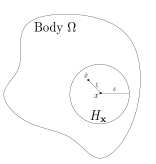
\includegraphics[width=0.8\textwidth]{figures/peridynamic}
	\caption{Point $\bm{x}$ in the body interacts with every point $\bm{\hat{x}}$ in its horizon $H_{\bm{x}}$}
\end{figure}
In the following, the relative position between two material points will be denoted 
\begin{equation}
\bm{\xi}=\hat{\bm{x}}-\bm{x}
\end{equation} 
and their relative displacement 
\begin{equation}
\bm{\eta}=\bm{u}(\hat{\bm{x}},t)-\bm{u}(\bm{x},t)
\end{equation}
In peridynamics, $\bm{x}$ interacts with every point $\bm{\hat{x}}$ within its horizon. The direct physical interaction between two points will be called a \textit{bond}, and in the special case of elastic interaction also \textit{spring}. The concept of a horizon is a very big difference to the classical theory where you only have contact forces between particles which are in direct contact.

It is common to assume that the horizon is defined with a positive number $\delta$ such that
\begin{equation}
\Vert \bm{\xi} \Vert > \delta \Rightarrow \bm{f}(\bm{\eta},\bm{\xi})=\bm{0} \qquad \forall \bm{\eta}
\end{equation}
This means that every particle only exerts a force on particles which are in a finite distance of $\delta$.

If the pairwise force function can be derived from a pairwise potential $\omega$, the material is said to be microelastic, i.e.
\begin{equation}
\bm{f}(\bm{\eta},\bm{\xi})=\frac{\partial \omega(\bm{\eta},\bm{\xi})}{\partial \bm{\eta}}
\end{equation}

For a linear elastic material,
\begin{equation}
\omega(\bm{\xi},\bm{\eta})=\frac{c(\bm{\xi})s^2\Vert\bm{\xi}\Vert}{2}
\end{equation}
where \begin{equation}
s=\frac{\Vert\bm{\eta}+\bm{\xi}\Vert-\Vert\bm{\xi}\Vert}{\Vert\bm{\xi}\Vert}
\end{equation} denotes the strain of a bond.
Thus the pairwise force function is
\begin{equation}
\bm{f}(\bm{\eta},\bm{\xi})=c(\bm{\xi})s
\end{equation}


\begin{equation}
\bm{f}(\bm{\xi,\eta})=\begin{cases}
\frac{\bm{\eta}+\bm{\xi}}{\Vert\bm{\eta}+\bm{\xi}\Vert}c(\bm{\xi})s & \Vert\bm{\xi}\Vert\leq\delta\\
\bm{0} & \Vert\bm{\xi}\Vert>\delta
\end{cases}
\end{equation}


The local strain energy density is
\begin{equation}
W = \frac{1}{2}\int_{H_{\bm{x}}} \omega(\bm{\eta},\bm{\xi})dV_{\bm{\xi}}
\end{equation}



\newpage
\subsection{Parameter}
For PMB material we need to specify two parameters $c$ and $s_0$.
We use a horizon of  $\delta = 4*\Delta x=4*0.0005=0.002$:
\subsubsection{2D plane stress}
From https://link.springer.com/content/pdf/10.1007\%2Fs10704-010-9442-4.pdf
\begin{align}
G_0 &= \frac{K_{Ic}^2}{E}=\frac{(50MPa\sqrt{m})^2}{200GPa}=12500Pa\cdot m\\
c&=\frac{6E}{\pi \delta^3(1-\nu)}=\frac{6*200GPa}{\pi *(0.002m)^3(1-0.3)}=6.820926\times10^{19} Pa/m^3\\
s_0&=\sqrt{\frac{4\pi G_0}{9E\delta}}=\sqrt{\frac{4\pi*12500Pa\cdot m}{9*200GPa*0.002m}}=0.0066055
\end{align}

\subsubsection{3D}
From http://www.sciencedirect.com/science/article/pii/S0045794905000805\\
Is $G_0$ correct??? Or do I need to use $\frac{E}{1-\nu^2}$???
\begin{align}
G_0 &= \frac{K_{Ic}^2}{E}=\frac{(50MPa\sqrt{m})^2}{200GPa}=12500Pa\cdot m\\
k &= \frac{E}{3(1-2\nu)}=\frac{200GPa}{3(1-2*0.3)}=165GPa\\
c&=\frac{18k}{\pi \delta^4}=\frac{18*165GPa}{\pi (0.002m)^4}=5.908627\times10^{22}Pa/m^4\\
s_0&=\sqrt{\frac{5G_0}{9k\delta}}=\sqrt{\frac{5*12500Pa\cdot m}{9*165GPa*0.002m}}=0.004587
\end{align}

\subsubsection{2D plane strain}
Like https://link.springer.com/content/pdf/10.1007\%2Fs10704-010-9442-4.pdf!
Not sure if correct!
\begin{align}
G_0 &= \frac{K_{Ic}^2(1-\nu^2)}{E}=\frac{(50MPa\sqrt{m})^2(1-0.3^2)}{200GPa}=11375Pa\cdot m\\
c&=\frac{6E}{\pi \delta^3(1-\nu-2\nu^2)}=\frac{6*200GPa}{\pi *(0.002m)^3(1-0.3-2*0.3^2)}=9.1820159\times10^{19} Pa/m^3\\
s_0&=\sqrt{\frac{4\pi G_0(1-\nu)}{9E\delta(1-\nu-2\nu^2)}}=\sqrt{\frac{4\pi*12500Pa\cdot m*(1-0.3)}{9*200GPa*0.002m*(1-0.3-2*0.3^2)}}=0.007664
\end{align}


\section{Stress Field}
$\sigma_\infty=\frac{0.007Pam^3}{1.25e-10m^3}=56MPa$ read from LAMMPS.\\
For $\theta = 0$:
\begin{align}
	\sigma(r) &= \frac{K_I}{\sqrt{2\pi r}}\\
	&=\frac{\beta \sigma_\infty\sqrt{\pi a}}{\sqrt{2\pi r}}\\
	&=\frac{1.12*\frac{0.007Pam^3}{1.25e-10m^3}*\sqrt{\pi*0.012m}}{\sqrt{2\pi r}}\\
	&=\frac{4.85827MPa\sqrt{m}}{\sqrt{r}}
\end{align}

\begin{figure}[hbtp]
	\centering
	\includegraphics[width=0.7\textwidth]{Skripte/stressComparison}
	\label{fig:stressComparison}
	\caption{For small r, both stresses coincide very well. For $radius>0.005$, the theoretical stress gets less accurate because the second order terms have been neglected. On the other hand, the LAMMPS stress approaches $\sigma_\infty$ which is physically correct.}
\end{figure}